\documentclass[11pt]{article}

\usepackage[spanish,es-nodecimaldot]{babel}
\usepackage{fontspec}
\usepackage{amsmath,amssymb}
\usepackage{booktabs}
\usepackage{array}
\usepackage{tabularx}
\usepackage{graphicx}
\usepackage{float}
\usepackage{caption}
\usepackage{xcolor}
\usepackage{listings}
\usepackage[hidelinks]{hyperref}

\graphicspath{{figuras/}}
\newcommand{\co}{\texorpdfstring{CO$_2$}{CO2}}
\DeclareMathOperator{\RMSE}{RMSE}

\lstset{
  basicstyle=\ttfamily\footnotesize,
  breaklines=true,
  breakatwhitespace=true,
  numbers=left,
  numberstyle=\tiny\color{gray},
  frame=single,
  showstringspaces=false,
  captionpos=b,
  extendedchars=true
}

\title{Modelo dinámico de generación de \co{} durante la
bioconversión con \textit{Hermetia illucens}:
del núcleo larvario de Eriksen al acople alimento--larva--lecho}
\author{}
\date{\today}

\begin{document}

\maketitle

\section*{Resumen}

Este trabajo formula y evalúa un modelo dinámico de caja gris para la
generación de dióxido de carbono durante la bioconversión de residuos
orgánicos con \textit{Hermetia illucens}. El punto de partida es el
núcleo larvario de Eriksen, expresado en equivalentes de carbono, que
conserva los balances de biomasa estructural, lípidos, mantenimiento y
costos respiratorios de crecimiento. Sobre ese núcleo se incorporan dos
componentes: una fuente microbiana asociada con la degradación del
alimento y un acople entre la disponibilidad de alimento y la
asimilación larvaria. El dióxido de carbono medido en cámara se
representa como la suma de las contribuciones larvaria y microbiana.

En ocho cierres de gas de los experimentos propios, el núcleo original
sin reajuste produjo un RMSE conjunto de $183{,}61$ ppm/min. El modelo
completo recalibrado redujo el error a $85{,}16$ ppm/min, equivalente a
una disminución de $53{,}6$\,\%. La reducción no debe atribuirse
exclusivamente al lecho: el ajuste conjunto incluye la recalibración de
la asimilación larvaria, el acople con el alimento y la nueva fuente
microbiana.

La transferencia a Laganaro, Bekker, Ermolaev, Schøn y Rossi muestra
capacidades y límites diferentes en cada estudio. El modelo propuesto
mejora algunos errores agregados, pero no reproduce universalmente el
efecto de dietas de baja calidad, la distribución temporal de los picos,
la partición microbiana ni el colapso a temperaturas extremas. El
resultado principal es, por tanto, una mejora local en los datos propios
y una representación explícita de las fuentes de \co{}, no una
superioridad general frente al modelo de Eriksen.

\section{Introducción}

La bioconversión con \textit{Hermetia illucens} transforma residuos
orgánicos en biomasa larvaria y un residuo estabilizado. Desde la
ingeniería ambiental, sin embargo, también es necesario cuantificar el
carbono que retorna a la atmósfera durante el proceso. La producción de
\co{} constituye un observable integrador de la respiración larvaria y
de la degradación microbiana del alimento. Por ello, un modelo útil debe
representar tanto la magnitud total del flujo como su evolución temporal
y su dependencia del sustrato.

El modelo dinámico de Eriksen describe el crecimiento y la respiración
de una larva mediante balances de carbono estructural y lipídico
\cite{eriksenDynamicModellingFeed2022}. Sus reproducciones de los
experimentos de Laganaro y Bekker muestran que el núcleo puede
representar trayectorias individuales de \co{} bajo condiciones
conocidas \cite{laganaroGrowthMetabolicPerformance2021a,
bekkerImpactSubstrateMoisture2021a}. No obstante, esas reproducciones
no constituyen validaciones independientes del presente trabajo, porque
los mismos escenarios intervinieron en la parametrización del modelo de
referencia.

Los experimentos de Ermolaev, Schøn y Rossi aportan condiciones de
transferencia diferentes: medición de emisiones totales, variación de
temperatura y comparación entre tratamientos y controles,
respectivamente \cite{ermolaevGreenhouseGasEmissions2019,
schonEffectTemperatureGrowth2024,
rossiEstimatingDynamicsGreenhouse2024a}. En conjunto, permiten examinar
si un modelo calibrado localmente conserva su capacidad predictiva al
cambiar el alimento, la humedad, la temperatura y el sistema de
observación.

El objetivo de este artículo es formular y evaluar un modelo de caja
gris para la generación de \co{} que conserve el núcleo de Eriksen e
incorpore explícitamente la relación
\[
\text{alimento}\longrightarrow
\text{larvas}+\text{lecho}\longrightarrow \text{\co{}}.
\]
Se distinguen tres preguntas: (i) cuánto del error proviene de aplicar
el núcleo original fuera de su dominio de calibración; (ii) cuánto
aporte representa el lecho microbiano en el total de cámara; y (iii) si
la disponibilidad de alimento permite explicar las diferencias entre
dietas sin sustituir los balances respiratorios originales.

La evaluación separa transferencia sin reajuste, recalibración y
comparación entre configuraciones. Una recalibración con datos propios
mide capacidad de ajuste; no equivale a una validación externa
independiente.

\section{Modelo dinámico}

\subsection{Sistema y fuentes de CO$_2$}

El sistema experimental se representa mediante dos fuentes acopladas: la respiración larvaria y la degradación microbiana del alimento o lecho. La tasa total de producción de CO$_2$ es
\begin{equation}
  R_{\mathrm{total}}(t)
  =
  R_{\mathrm{lar}}(t)+R_{\mathrm{mic}}(t).
  \label{eq:fuentes-totales}
\end{equation}
Esta descomposición permite contrastar por separado los controles sin larvas, las larvas en ayuno y los tratamientos completos antes de evaluar el sistema integrado.

\subsection{Estados larvarios}

La larva se describe mediante tres compartimentos: asimilados disponibles $A(t)$, biomasa estructural $B(t)$ y reservas lipídicas $L(t)$. El crecimiento medido corresponde a una observación agregada de la biomasa larvaria, de modo que no identifica por sí solo cada compartimento.

\subsection{Alimentación y asimilación}

La ingesta dependerá de la dieta, la disponibilidad del sustrato y el estado de desarrollo. La fracción asimilada alimenta el compartimento $A$, desde el cual se atienden mantenimiento, síntesis de biomasa estructural y acumulación de lípidos. La formulación completa se fijará después de verificar las unidades de todos los parámetros.

\subsection{Crecimiento y respiración larvaria}

La producción larvaria de CO$_2$ se descompone en mantenimiento y costos respiratorios de síntesis:
\begin{equation}
  R_{\mathrm{lar}}(t)
  =
  r_{\mathrm{m}}(t)
  +\gamma_B\,\dot B(t)
  +\gamma_L\,\max\{\dot L(t),0\}.
  \label{eq:respiracion-larvaria}
\end{equation}
No se asigna producción de CO$_2$ a la movilización neta de lípidos; esa contribución queda asociada con el mantenimiento y con los flujos de síntesis efectivamente positivos.

\subsection{Módulo microbiano del lecho}

El lecho se representa mediante materia orgánica degradable $D_M(t)$ y una variable microbiana efectiva $X(t)$. La degradación sigue una cinética de disponibilidad:
\begin{equation}
  r_{\mathrm{deg}}(t)
  =
  k_{\mathrm{deg}}X(t)
  \frac{D_M(t)}{K_{SM}+D_M(t)},
  \qquad
  R_{\mathrm{mic}}(t)
  =
  Y_{\mathrm{CO_2}}r_{\mathrm{deg}}(t).
  \label{eq:modulo-microbiano}
\end{equation}
Los controles de alimento sin larvas son la restricción principal de este módulo.

\subsection{Balance de la cámara de medición}

La variable observada por el sensor es la pendiente temporal de la concentración en la cámara cerrada. Si $R_{\mathrm{total}}$ está en mol por unidad de tiempo,
\begin{equation}
  \frac{dC_{\mathrm{ppm}}}{dt}
  =
  10^6\,\frac{R_uT}{P_{\mathrm{atm}}V_{\mathrm{air}}}\,
  R_{\mathrm{total}}(t).
  \label{eq:balance-camara}
\end{equation}
Las tasas experimentales se recalcularán intervalo por intervalo a partir de las marcas temporales reales; no se aplicará un factor global de conversión.

\subsection{Observables e identificabilidad}

\begin{center}
\begin{tabular}{lll}
\toprule
Medición & Fuente dominante & Restricción del modelo \\
\midrule
Alimento D1 sin larvas & $R_{\mathrm{mic}}$ & Módulo microbiano D1 \\
Alimento D4 sin larvas & $R_{\mathrm{mic}}$ & Módulo microbiano D4 \\
Larvas solas en ayuno & $R_{\mathrm{lar}}$ & Mantenimiento larvario \\
Alimento D1 con larvas & $R_{\mathrm{total}}$ & Acoplamiento en D1 \\
Alimento D4 con larvas & $R_{\mathrm{total}}$ & Acoplamiento en D4 \\
Crecimiento D1 y D4 & Biomasa larvaria & Crecimiento agregado \\
\bottomrule
\end{tabular}
\end{center}

La diferencia tratamiento--control no se interpretará automáticamente como respiración larvaria, porque las larvas también pueden modificar la actividad microbiana del lecho. La validación debe combinar componentes independientes, sistema integrado y transferencia a datos externos.

\section{Parámetros, unidades y procedencia}

\subsection{Parámetros del núcleo larvario}

\begin{table}[H]
\centering
\small
\caption{Parámetros principales del núcleo de Eriksen y su tratamiento
en la calibración propia.}
\begin{tabularx}{\textwidth}{l l X l}
\toprule
Símbolo & Unidades & Significado & Tratamiento \\
\midrule
$B$ & mg C/larva & Biomasa estructural & Estado \\
$L_{\mathrm{tot}}$ & mg C/larva & Lípidos totales & Estado \\
$a_{\max}$ & d$^{-1}$ & Asimilación máxima de referencia &
Calibrado: $1{,}4995$ \\
$\alpha,\beta$ & -- & Factores de las funciones de crecimiento y
desarrollo & Heredados \\
$Y_B$ & -- & Eficiencia de conversión a biomasa estructural &
Fijo: $0{,}44$ \\
$Y_L$ & -- & Eficiencia de conversión a lípidos &
Fijo: $0{,}42$ \\
$m$ & d$^{-1}$ & Coeficiente de mantenimiento &
Fijo: $0{,}08$ \\
$B_{\max,0}$ & mg C & Escala de biomasa estructural máxima &
Heredado: $39{,}69$ \\
$t_{p,\min}$ & d & Umbral mínimo de desarrollo &
$8{,}5$ desde montaje \\
$\rho$ & mg C/d & Escala del costo máximo de crecimiento &
Calibrado: $4{,}395$ \\
$\delta_I$ & d & Duración de instares & Heredado \\
$\delta_{CL}$ & -- & Fracción de carbono en lípidos &
Heredado: $0{,}79$ \\
$\delta_{CB}$ & -- & Fracción de carbono en biomasa &
Heredado: $0{,}49$ \\
\bottomrule
\end{tabularx}
\end{table}

La conservación del núcleo no implica conservar idénticos todos sus
valores numéricos. En la calibración propia se ajustan $a_{\max}$,
$\rho$ y $f_{D4}$, mientras $Y_B$, $Y_L$ y $m$ permanecen congelados.
Por tanto, no es correcto afirmar que el modelo propuesto eliminó los
costos de crecimiento o el mantenimiento.

Esta distinción también explica parte de las diferencias externas. En
la reproducción de Laganaro, Eriksen emplea $Y_B=0{,}44$ y $m=0{,}08$
para la dieta de alta calidad, pero $Y_B=0{,}76$ y $m=0{,}23$ para el
escenario con 75\,\% de lodos. Esos cambios aumentan los costos
metabólicos asociados con la dieta de baja calidad. El modelo propuesto
actual, con $Y_B$ y $m$ congelados, no reproduce ese mecanismo.

\subsection{Parámetros del alimento y del lecho}

\begin{table}[H]
\centering
\small
\caption{Parámetros de la extensión alimento--lecho.}
\begin{tabularx}{\textwidth}{l l X l}
\toprule
Símbolo & Unidades & Significado & Valor u origen \\
\midrule
$D_C$ & g C/cámara & Carbono disponible del alimento & Estado \\
$X$ & g C/cámara & Biomasa microbiana & Estado \\
$f_d$ & -- & Disponibilidad integral de la dieta &
D1: $1$; D4: $0{,}8047$ \\
$K_D$ & g C & Semisaturación del acople alimento--larva &
Fijo: $2$ en tratamientos \\
$k_{\mathrm{ref}}$ & d$^{-1}$ & Cinética microbiana de referencia &
D1: $0{,}6086$; D4: $1{,}0$ \\
$K_{SM}$ & g C & Semisaturación de degradación & Fijo: $50$ \\
$Y_X$ & -- & Rendimiento de biomasa microbiana & Fijo: $0{,}4$ \\
$Y_{C,\mathrm{mic}}$ & -- & Fracción degradada emitida como \co{} &
Fijo: $0{,}4$ \\
$Q_{10}$ & -- & Factor de dependencia térmica & Fijo: $2$ \\
$T_{\mathrm{ref}}$ & $^\circ$C & Temperatura de referencia &
Fijo: $25$ \\
$\theta_d$ & -- & Humedad efectiva adimensional &
Según escenario \\
$K_\theta$ & -- & Semisaturación por humedad & Fijo: $0{,}15$ \\
$\delta_{CS}$ & -- & Fracción de carbono disponible del sustrato &
D1: $0{,}95$; D4: $0{,}2483$ \\
\bottomrule
\end{tabularx}
\end{table}

El valor $a_{\max}=1{,}4995$ d$^{-1}$ se encuentra próximo a su cota
superior. También $k_{\mathrm{ref}}(D4)=1$ y
$\delta_{CS}(D1)=0{,}95$ alcanzan sus fronteras superiores. Estos
resultados se reportan como tales: no se eliminan ni se sustituyen por
valores más favorables. Señalan que algunos parámetros absorben
limitaciones estructurales o información insuficiente.

\subsection{Qué se calibró en cada etapa}

La primera etapa utiliza controles sin larvas para estimar
$k_{\mathrm{ref}}$ y $\delta_{CS}$ por dieta. La segunda congela esos
parámetros microbianos y ajusta $a_{\max}$, $\rho$ y $f_{D4}$ contra
crecimiento inicial y ocho cierres de gas. El ajuste de crecimiento se
restringe a días $\leq8$; la fase tardía se conserva como diagnóstico.

La mejora obtenida en la segunda etapa corresponde al sistema completo.
No identifica por sí sola la contribución causal del lecho, porque la
recalibración larvaria y el acople con el alimento cambian
simultáneamente.

\section{Resultados}

\subsection{Verificación y alcance del núcleo de referencia}

La implementación del núcleo se contrastó con las ecuaciones y los
escenarios publicados por Eriksen. Esta verificación comprueba que el
código reproduce el modelo de referencia; no demuestra que el modelo
sea transferible sin reajuste a otros alimentos o sistemas de medición.

En Laganaro, la reproducción del \co{} individual presenta RMSE entre
$2{,}32$ y $3{,}54$ mg \co{}/d/larva. En Bekker, el intervalo es
$2{,}29$--$4{,}58$ mg \co{}/d/larva. Como esos escenarios ya
intervinieron en la parametrización original, se interpretan como
reproducción del modelo y no como validación independiente.

\subsection{Ajuste de calibración en los datos propios}

El núcleo original se aplicó sin lecho y sin reajuste a los ocho cierres
de gas. La tabla compara las observaciones con las predicciones del
modelo original y del modelo completo propuesto.

\begin{table}[H]
\centering
\small
\caption{Cierres propios y predicciones de la calibración completa;
no son predicciones fuera de muestra. Los valores precedidos por $\geq$
son cotas inferiores por saturación. Unidades: ppm/min.}
\begin{tabular}{l c r r r}
\toprule
Dieta & Día & Observado & Eriksen & Propuesto \\
\midrule
D1 & 6, R1 & $\geq670{,}56$ & $273{,}71$ & $469{,}38$ \\
D1 & 6, R2 & $\geq474{,}23$ & $273{,}71$ & $469{,}38$ \\
D1 & 8     & $\geq311{,}82$ & $315{,}69$ & $450{,}34$ \\
D1 & 10    & $285{,}57$     & $303{,}38$ & $290{,}47$ \\
D4 & 6     & $228{,}52$     & $247{,}59$ & $323{,}89$ \\
D4 & 8     & $\geq383{,}67$ & $308{,}53$ & $331{,}79$ \\
D4 & 10    & $104{,}11$     & $306{,}22$ & $144{,}13$ \\
D4 & 14    & $79{,}11$      & $236{,}72$ & $143{,}21$ \\
\bottomrule
\end{tabular}
\end{table}

\begin{table}[H]
\centering
\caption{RMSE censurado de calibración, calculado sobre los mismos
ocho cierres utilizados en el ajuste.}
\begin{tabular}{l r r r}
\toprule
Dieta & Eriksen & Propuesto & Reducción \\
 & (ppm/min) & (ppm/min) & del error \\
\midrule
D1 & $222{,}49$ & $100{,}65$ & $54{,}8$\,\% \\
D4 & $133{,}88$ & $66{,}14$ & $50{,}6$\,\% \\
Conjunto & $183{,}61$ & $85{,}16$ & $53{,}6$\,\% \\
\bottomrule
\end{tabular}
\end{table}

En la calibración completa, los cuatro cierres no saturados dan un RMSE
de $60{,}89$ ppm/min. La cobertura de las cuatro cotas saturadas es
$1/4$; por tanto, la reducción del RMSE no implica que todas las
predicciones superen los límites instrumentales observados.

El RMSE de los controles sin larvas es $7{,}82$ ppm/min para D1 y
$7{,}95$ ppm/min para D4. El módulo microbiano representa
satisfactoriamente esos controles, pero su contribución predicha al
tratamiento no explica por sí sola toda la diferencia entre modelos.

\subsection{Validación cruzada interna}

La capacidad predictiva se evaluó mediante siete pliegues agrupados por
dieta y día. Los dos cierres de D1 del día 6 se excluyeron conjuntamente.
En cada pliegue se retiraron también el control y las observaciones de
crecimiento del día evaluado, y se recalibraron las etapas 1 y 2. Se
compararon el modelo original sin reajuste (E0), el núcleo recalibrado sin
lecho (R), el lecho aditivo (A) y el modelo acoplado (C). Cada cierre de
tratamiento fue predicho una única vez fuera de la calibración.

\begin{table}[H]
\centering
\small
\caption{Desempeño fuera de calibración. El RMSE censurado incluye los
ocho cierres; el RMSE exacto utiliza únicamente los cuatro no saturados.}
\begin{tabular}{l r r r}
\toprule
Modelo & RMSE censurado & RMSE exactos & Cobertura saturados \\
 & (ppm/min) & (ppm/min) & (\%) \\
\midrule
E0 & $183{,}61$ & $128{,}81$ & $25$ \\
R  & $164{,}21$ & $151{,}34$ & $50$ \\
A  & $154{,}21$ & $155{,}44$ & $50$ \\
C  & $124{,}94$ & $137{,}20$ & $25$ \\
\bottomrule
\end{tabular}
\label{tab:validacion_cruzada}
\end{table}

El modelo C presentó el menor RMSE censurado conjunto. Frente a E0, la
reducción puntual fue $31{,}95$\,\%; frente a R y A fue $23{,}92$\,\% y
$18{,}98$\,\%, respectivamente. No obstante, en los cuatro cierres no
saturados, C obtuvo un error $6{,}51$\,\% mayor que E0. Tampoco aumentó la
cobertura de las cotas saturadas respecto de E0.

Las predicciones fuera de muestra muestran dos limitaciones localizadas.
C subestimó los dos cierres de D1 del día 6 y sobreestimó los puntos
posteriores al pico: el residuo fue $+146{,}81$ ppm/min en D1, día 10, y
$+200{,}07$ ppm/min en D4, día 14. Por tanto, la reducción conjunta no
implica una mejora uniforme a lo largo del experimento.

El bootstrap exploratorio por dieta y día, con 5000 remuestreos, produjo
para C un RMSE censurado mediano de $124{,}94$ ppm/min y un rango percentil
de $75{,}64$--$157{,}98$ ppm/min. La reducción frente a E0 presentó un
rango de $-82{,}19$\,\% a $52{,}46$\,\%, y fue positiva en $80{,}5$\,\% de
los remuestreos. Estos porcentajes describen el remuestreo de siete días;
no constituyen una probabilidad de superioridad ni un intervalo de
confianza de validación independiente.

\subsection{Sensibilidad e identificabilidad}

En la calibración canónica, el modelo estimó $154{,}90$ g de \co{} en D1 y
$87{,}96$ g en D4 durante 14 días. La suma aritmética de ambos escenarios
independientes fue $242{,}86$ g. La sensibilidad local se evaluó mediante
perturbaciones de $\pm10$\,\%; en los parámetros situados en una cota solo
se perturbó hacia el interior del dominio.

\begin{table}[H]
\centering
\small
\caption{Máximo efecto local por parámetro. El cambio del acumulado usa la
suma de los escenarios D1 y D4; el cambio del RMSE se expresa en ppm/min.}
\begin{tabular}{l r r}
\toprule
Parámetro & Cambio máximo del \co{} total & Cambio máximo del RMSE \\
\midrule
$a_{\max}$       & $5{,}49$\,\% & $13{,}72$ \\
$k_{\mathrm{ref,D1}}$ & $3{,}06$\,\% & $2{,}57$ \\
$\delta_{CS,D4}$ & $2{,}75$\,\% & $5{,}36$ \\
$f_{D4}$         & $1{,}70$\,\% & $7{,}24$ \\
$\delta_{CS,D1}$ & $1{,}41$\,\% & $1{,}11$ \\
$\rho$           & $0{,}18$\,\% & $0{,}26$ \\
$k_{\mathrm{ref,D4}}$ & $0{,}10$\,\% & $0{,}19$ \\
\bottomrule
\end{tabular}
\label{tab:sensibilidad_local}
\end{table}

El acumulado fue localmente poco sensible a $\rho$. El perfil de costo,
reoptimizando $a_{\max}$ y $f_{D4}$, confirmó que su límite superior no
queda bien identificado. En la malla evaluada, los perfiles con aumento de
costo $\leq1$\,\% correspondieron a $\rho$ entre $4{,}395$ y $15$ y
produjeron entre $237{,}06$ y $243{,}00$ g de \co{} en el escenario
conjunto. Esta región es una comparación exploratoria, no un intervalo de
confianza.

El parámetro $a_{\max}$ tuvo el mayor efecto local sobre el ajuste. Su
perfil favoreció valores próximos a la cota superior: el costo aumentó
$4{,}75$\,\% al fijar $a_{\max}=1{,}45$ y $11{,}14$\,\% al fijarlo en
$1{,}40$. En consecuencia, el valor calibrado se reporta como un óptimo en
frontera dentro del rango declarado, no como una estimación fisiológica
precisa y libre de restricciones.

\subsection{Por qué Eriksen no describe apropiadamente los datos propios}

El desempeño del modelo original combina tres limitaciones.

\paragraph{Ausencia de la fuente microbiana.}
El núcleo original produce únicamente \co{} larvario, mientras el
observable propio corresponde al total de cámara. Los controles confirman
que existe una señal sin larvas. No obstante, añadir una fuente aditiva
no basta para corregir toda la discrepancia.

\paragraph{Transferencia de parámetros fuera de su dominio.}
Los valores originales se aplicaron sin recalibrar a otro alimento,
otra densidad de larvas y otro sistema experimental. En D1, día 6, la
predicción original de $273{,}71$ ppm/min queda aproximadamente
$59$\,\% por debajo de la cota de $670{,}56$ ppm/min. En D4 ocurre lo
contrario al final del experimento: el modelo predice
$306{,}22$ ppm/min frente a $104{,}11$ ppm/min en el día 10 y
$236{,}72$ ppm/min frente a $79{,}11$ ppm/min en el día 14.

\paragraph{Ausencia de acople dinámico con el alimento.}
En el modelo original, $a_d=a_{\max}$ mientras no se active el límite de
desarrollo. El alimento no reduce progresivamente la asimilación a
medida que se consume. En cambio, el modelo propuesto utiliza
$f_dD_C/(K_D+D_C)$, lo que permite una disminución más temprana del
\co{} en D4 y una trayectoria diferente entre dietas.

El diagnóstico neto larvario del modelo propuesto todavía presenta un
RMSE conjunto de $108{,}15$ ppm/min. Por tanto, la mejora total no debe
interpretarse como una reconstrucción perfecta de la respiración
individual.

\subsection{Descomposición del \co{} predicho}

La contribución microbiana predicha en D1 aumenta desde $9{,}6$\,\% en
el día 6 hasta $13{,}5$\,\% en el día 8 y $27{,}9$\,\% en el día 10.
En D4 disminuye desde $8{,}0$\,\% y $4{,}6$\,\% en los días 6 y 8
hasta $0{,}7$\,\% y aproximadamente $0{,}02$\,\% en los días 10 y 14.

Estas diferencias muestran que el lecho tiene un papel dinámico y
dependiente de la dieta. Sin embargo, la partición tratamiento menos
control no siempre es físicamente interpretable: en D4, día 14, esa
diferencia observacional es $-28{,}9$ ppm/min. El resultado refuerza la
necesidad de modelar el sistema acoplado en lugar de asignar
directamente toda la diferencia a las larvas.

\begin{figure}[H]
\centering
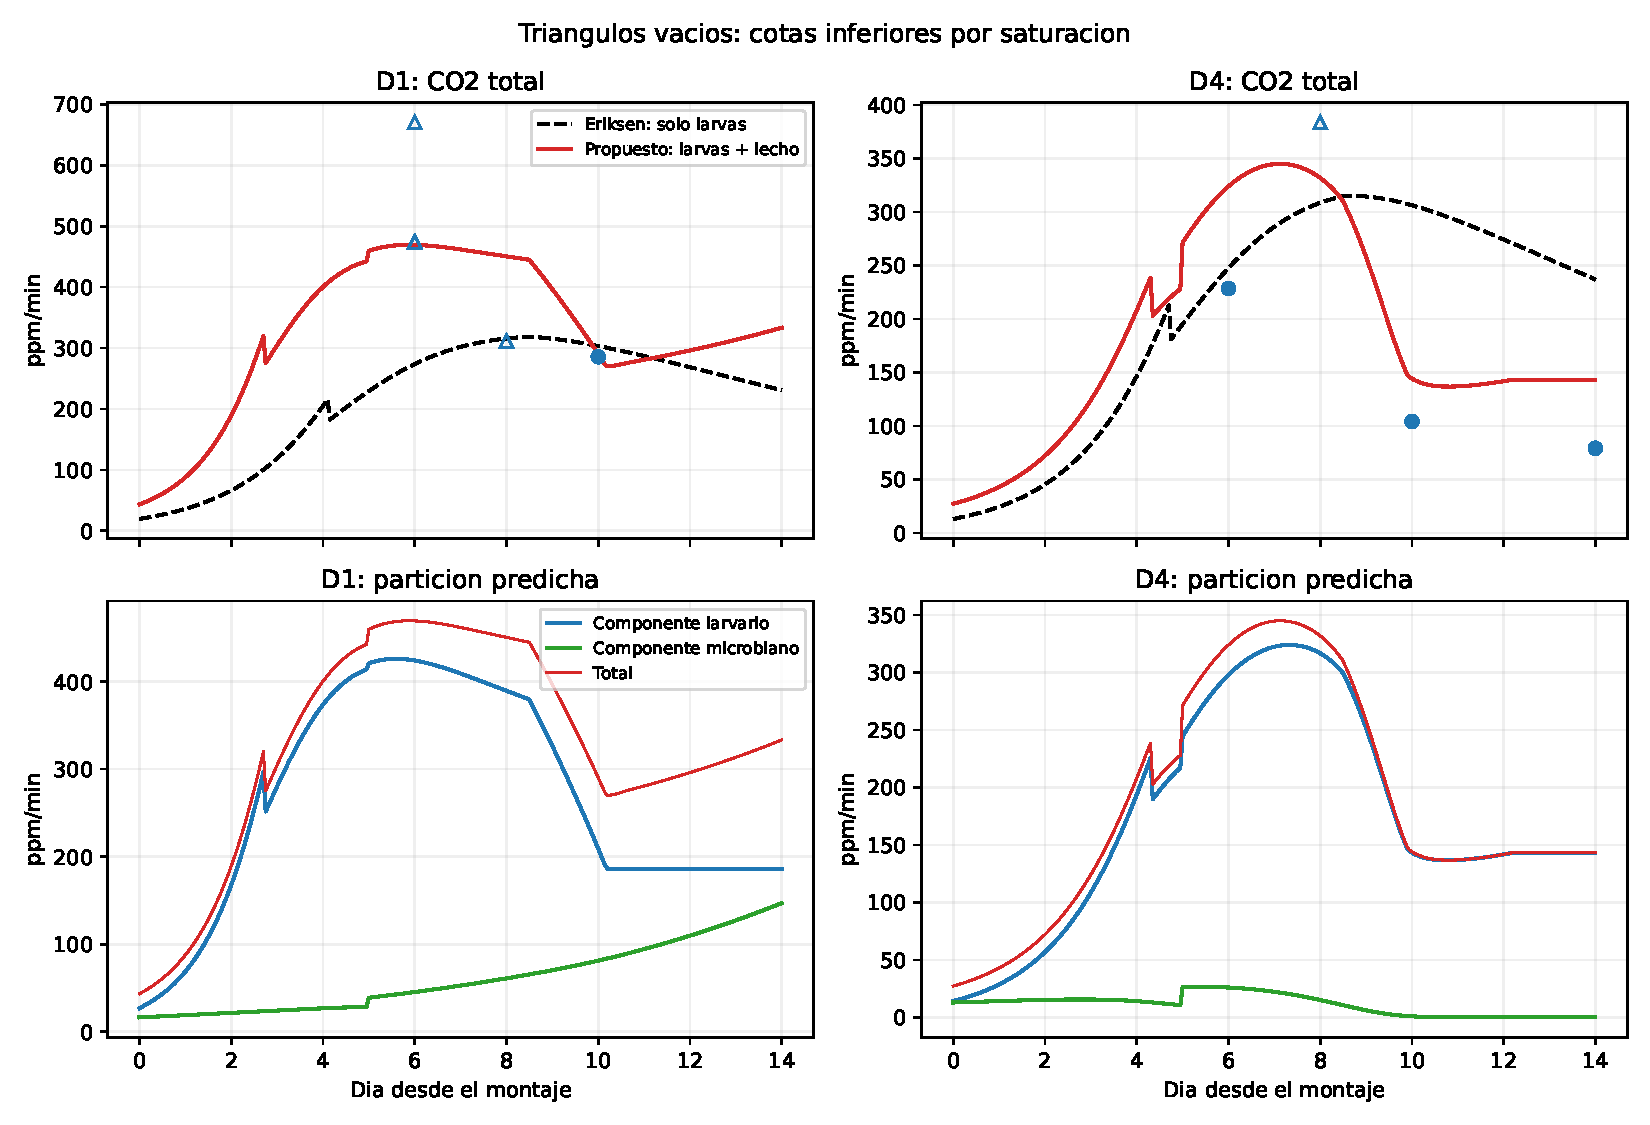
\includegraphics[width=\textwidth]{datos_propios_modelos.pdf}
\caption{Datos propios. Paneles superiores: Eriksen original y modelo
completo propuesto frente a los cierres observados. Paneles inferiores:
descomposición del modelo propuesto en componentes larvario y
microbiano. Los triángulos vacíos representan cotas inferiores por
saturación.}
\label{fig:datos_propios}
\end{figure}

\subsection{Transferencia externa}

\paragraph{Laganaro.}
Para la dieta sin lodos, el máximo específico observado es
$0{,}35$ d$^{-1}$ y el propuesto $0{,}42$ d$^{-1}$, con un error de
$+20$\,\%. Con 75\,\% de lodos, el observado aumenta a $0{,}64$ d$^{-1}$,
mientras el propuesto disminuye a $0{,}30$ d$^{-1}$, con un error
aproximado de $-52$\,\%. El factor $f_{D4}$ reduce disponibilidad, pero
no representa el aumento de costos metabólicos de una dieta de baja
calidad.

\paragraph{Bekker.}
El RMSE individual agrupado del modelo propuesto es
$1{,}50$ mg C/d/larva; por humedad, varía entre $1{,}19$ y
$1{,}76$ mg \co{}/d/larva. El intervalo correspondiente de Eriksen es
$2{,}29$--$4{,}58$ mg \co{}/d/larva. Sin embargo, el modelo propuesto
anticipa el pico individual entre $2{,}56$ y $7{,}50$ d, frente a
$0{,}67$--$2{,}59$ d en Eriksen.

El modelo propuesto reproduce algunos acumulados totales por
compensación de errores, pero no la partición de fuentes. Predice una
fracción microbiana aproximada de $66$--$67$\,\% en todas las humedades,
mientras la observada disminuye desde $78{,}1$\,\% hasta
$28{,}4$\,\%. El RMSE del total varía entre $0{,}49$ y
$1{,}80$ g C/d.

\paragraph{Ermolaev.}
En los días 2, 7 y 11, los flujos observados son $2{,}53$, $8{,}04$ y
$5{,}58$ mg/min. El modelo propuesto predice $4{,}69$, $9{,}04$ y
$4{,}98$ mg/min, con RMSE de $1{,}42$ mg/min, frente a
$1{,}83$ mg/min de Eriksen. No obstante, el acumulado propuesto es
$116{,}4$ g/kg FW, un $26$\,\% superior al observado de
$92{,}4$ g/kg FW, mientras Eriksen predice $75{,}8$ g/kg FW, un
$18$\,\% inferior. El pico propuesto ocurre en el día $5{,}1$, antes
del máximo observado alrededor del día 7.

\paragraph{Schøn.}
A $27{,}0$, $35{,}3$, $39{,}4$ y $41{,}9$ $^\circ$C, los totales
observados son $50$, $54{,}5$, $53$ y $24$ L/kg. El modelo propuesto
predice $81{,}6$, $90{,}3$, $98{,}2$ y $104{,}8$ L/kg, con errores de
$+63$\,\%, $+66$\,\%, $+85$\,\% y $+337$\,\%. El término $Q_{10}$
microbiano incrementa la emisión con la temperatura y no representa el
colapso observado a $41{,}9$ $^\circ$C.

\paragraph{Rossi.}
El modelo propuesto acumula $31{,}07$ g de \co{} total y
$11{,}05$ g en el control, con una diferencia neta de $20{,}02$ g.
Los valores netos observados son $5{,}55$, $32{,}38$ y $37{,}30$ g.
El RMSE neto disminuye desde $23{,}27$ g con Eriksen hasta
$14{,}84$ g con el propuesto, pero ninguno reproduce adecuadamente las
tres corridas. Además, el pico total propuesto ocurre en el día
$10{,}34$, frente a los días 5--7 observados.

\begin{figure}[H]
\centering
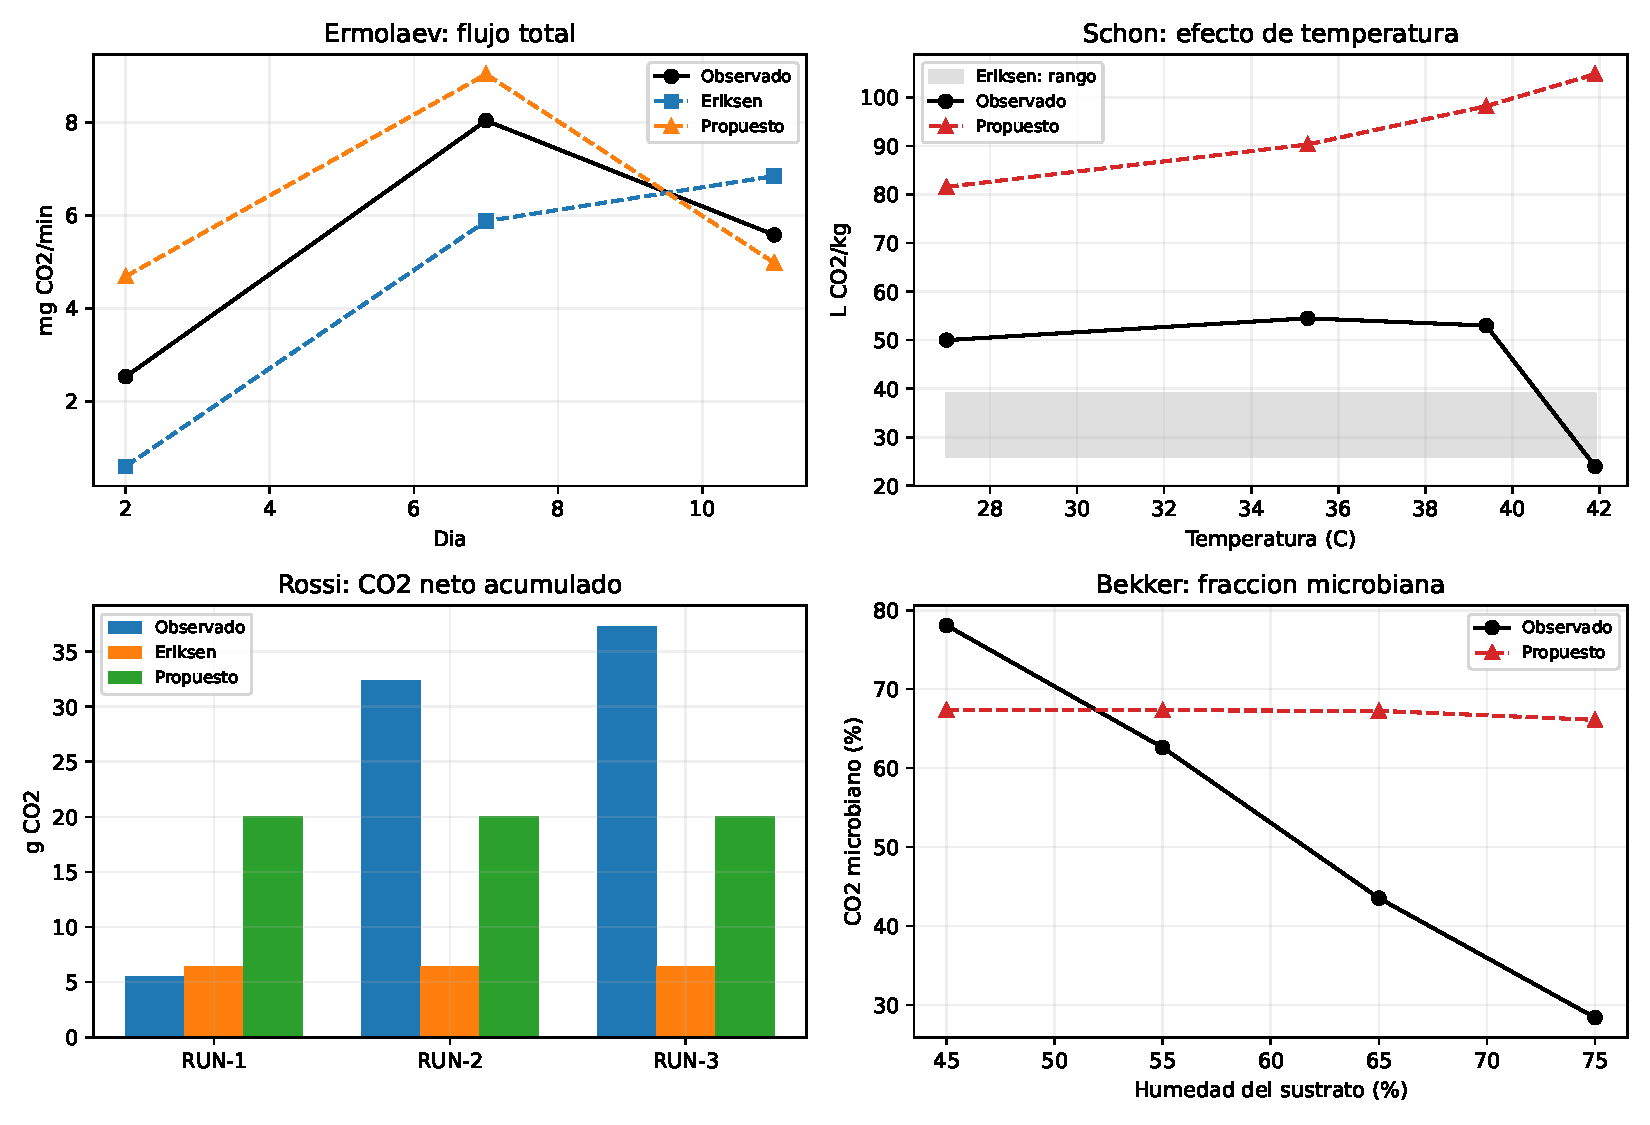
\includegraphics[width=\textwidth]{comparacion_externa.pdf}
\caption{Comparación externa de los observables publicados. Cada panel
conserva sus propias unidades y no debe interpretarse como una escala
común entre estudios.}
\label{fig:comparacion_externa}
\end{figure}

\begin{figure}[H]
\centering
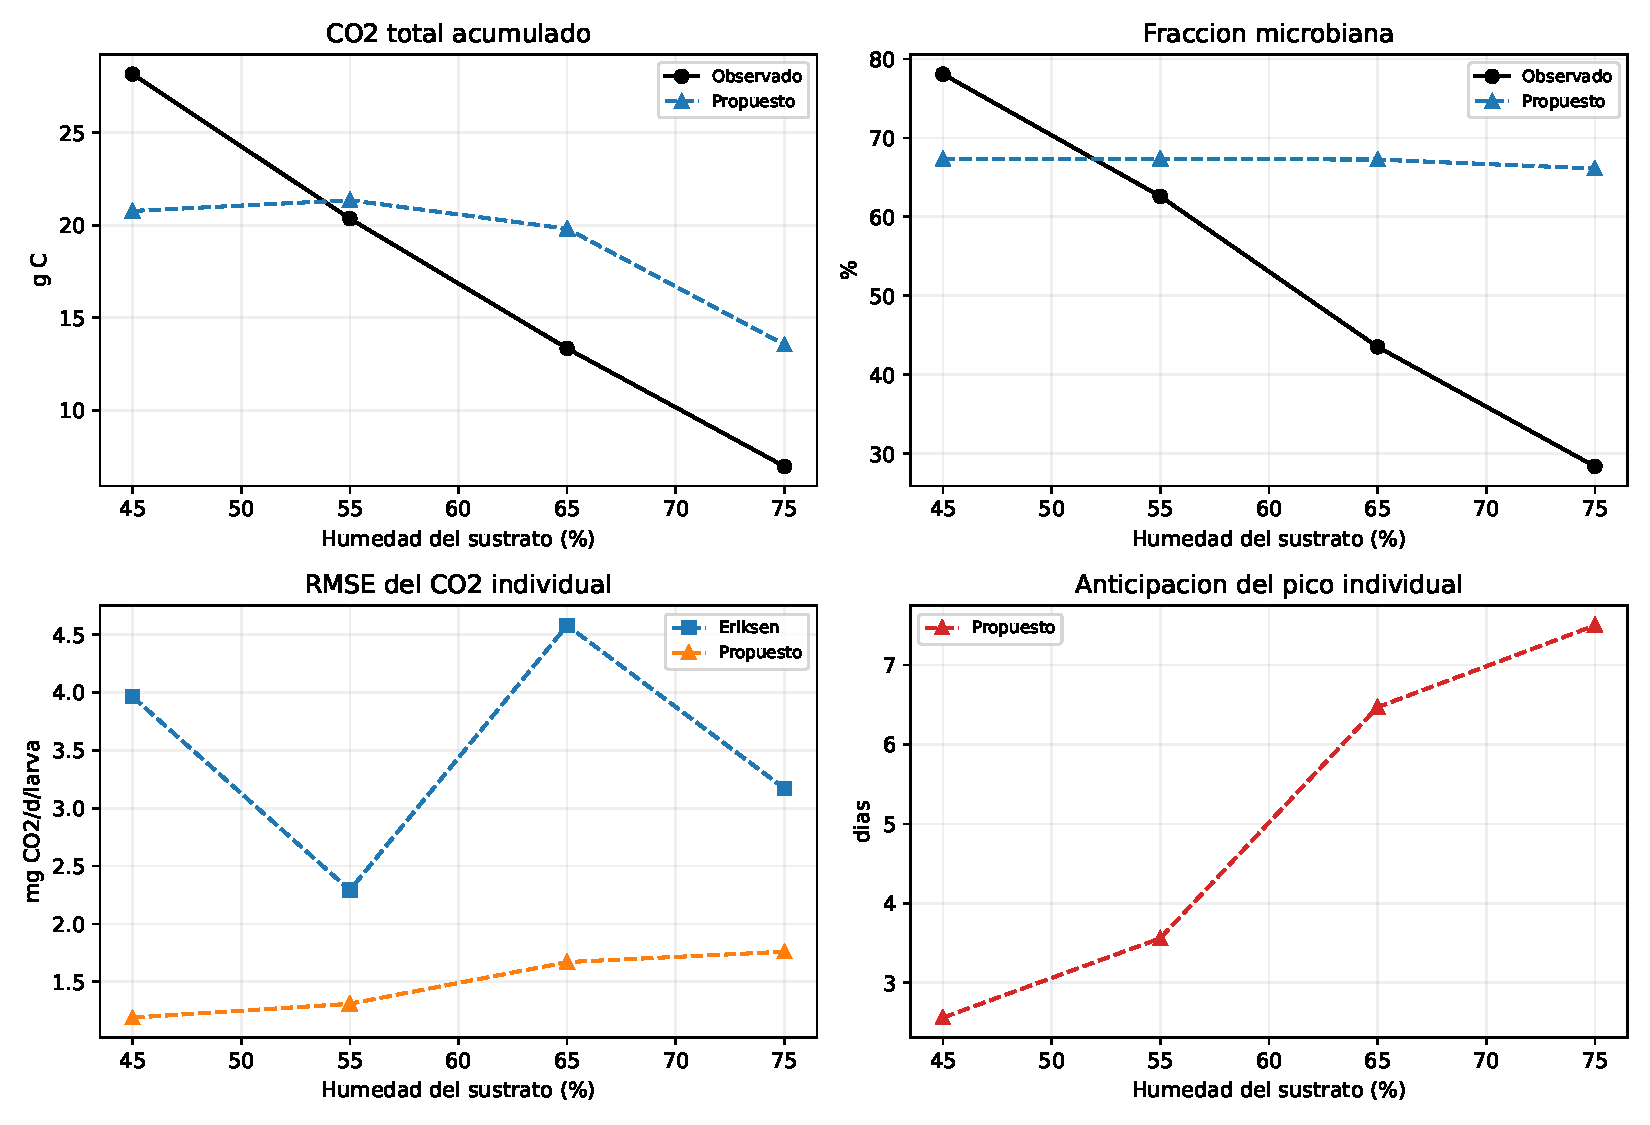
\includegraphics[width=\textwidth]{bekker_comparacion.pdf}
\caption{Evaluación detallada con Bekker: acumulado total, fracción
microbiana, error individual y anticipación del pico. La coincidencia
en algunos acumulados no implica una reproducción correcta de la
dinámica o de la partición entre fuentes.}
\label{fig:bekker}
\end{figure}

\subsection{Síntesis comparativa}

\begin{table}[H]
\centering
\small
\caption{Interpretación comparativa por estudio.}
\begin{tabularx}{\textwidth}{l X X}
\toprule
Estudio & Resultado favorable & Limitación principal \\
\midrule
Datos propios & Reduce el RMSE censurado $53{,}6$\,\% en calibración
y $31{,}95$\,\% en validación interna &
No mejora el RMSE exacto conjunto; el bootstrap exploratorio incluye
reducciones negativas \\
Laganaro & Eriksen reproduce el aumento de \co{} con baja calidad &
El propuesto no modifica $Y_B$ ni $m$ con la dieta \\
Bekker & El propuesto reduce el RMSE individual &
Anticipa picos y mantiene casi constante la fracción microbiana \\
Ermolaev & El propuesto reduce el RMSE de las tasas &
Sobrestima el acumulado y anticipa el pico \\
Schøn & Eriksen queda más cerca del rango observado &
El $Q_{10}$ propuesto impide representar el colapso térmico \\
Rossi & El propuesto reduce el RMSE neto agregado &
Ninguno reproduce las tres corridas ni el momento del pico \\
\bottomrule
\end{tabularx}
\end{table}

\section{Discusión}

\subsection{El modelo propuesto conserva el núcleo de Eriksen}

La diferencia estructural principal no consiste en sustituir la
respiración larvaria. Los términos $r_{C,m}$, $r_{C,B}$ y $r_{C,L}$
permanecen activos y continúan dependiendo de $m$, $Y_B$ y $Y_L$. El
modelo propuesto añade un estado microbiano y una dependencia de la
asimilación respecto del alimento disponible.

Por esta razón, los cambios de resultados entre estudios no pueden
explicarse únicamente por ``agregar el lecho''. En los datos propios
también cambian $a_{\max}$, $\rho$ y el factor dietario. Además, el
acople modifica la trayectoria larvaria a través de $D_C$, de modo que
el componente microbiano y el componente larvario dejan de ser
independientes.

\subsection{Interpretación del ajuste y de la validación interna}

En la calibración completa, el RMSE censurado conjunto disminuyó de
$183{,}61$ a $85{,}16$ ppm/min, equivalente a $53{,}6$ %. Este
resultado evidencia una mayor capacidad de ajuste del modelo completo
recalibrado, pero no constituye por sí solo evidencia predictiva fuera
de muestra.

En la validación cruzada interna agrupada por dieta y día, el modelo
acoplado redujo el RMSE censurado de $183{,}61$ a $124{,}94$ ppm/min,
una reducción puntual de $31{,}95$ % frente a Eriksen original. Sin
embargo, no mejoró el RMSE de los cierres exactos, que fue $137{,}20$
frente a $128{,}81$ ppm/min, ni la cobertura conjunta de las cotas
saturadas, que permaneció en $25$ %. Además, subestimó los dos cierres
de D1 en el día 6 y sobreestimó los cierres tardíos de D1 y D4.

El remuestreo bootstrap exploratorio confirmó una incertidumbre amplia:
los percentiles $2{,}5$ y $97{,}5$ de la reducción del RMSE censurado
frente a Eriksen fueron $-82{,}19$ y $52{,}45$ %, respectivamente.
Como este rango incluye reducciones negativas, la mejoría puntual no
debe interpretarse como superioridad predictiva concluyente. Tampoco
permite atribuir por separado los residuos restantes a una fuente
larvaria o microbiana específica.

\subsection{Ventajas y límites frente a estudios externos}

Los resultados externos impiden afirmar superioridad universal. En
Laganaro, la parametrización original de $Y_B$ y $m$ captura un efecto
de calidad dietaria que el factor de disponibilidad no reproduce. En
Bekker, la reducción del error individual convive con picos anticipados
y una partición microbiana casi invariante frente a la humedad.

En Ermolaev, el modelo propuesto mejora las tasas puntuales pero empeora
el sesgo del acumulado. En Schøn, el aumento monótono inducido por
$Q_{10}$ resulta incompatible con el colapso a alta temperatura. En
Rossi, una menor distancia agregada no equivale a reproducir la
variabilidad entre corridas ni el momento del pico.

Estas discrepancias muestran que un RMSE menor puede coexistir con una
dinámica o una partición incorrectas. La evaluación debe combinar
errores puntuales, acumulados, momentos de los picos y fracciones de
las fuentes.

\subsection{Descomposición controlada de la mejora}

La comparación entre Eriksen original, el núcleo recalibrado, el lecho
aditivo y el modelo acoplado permitió separar contablemente los
componentes de la reducción del error en calibración. La recalibración
del núcleo aportó $55{,}8$ % de la reducción total, la adición de
\co{} microbiano $12{,}7$ % y el acople con la disponibilidad de
alimento $31{,}5$ %. Por construcción, el lecho aditivo conserva la
trayectoria larvaria; en cambio, el acople la modifica mediante
$f_d\Phi_D(D_C)$.

Esta descomposición no identifica efectos causales independientes. La
recalibración modifica parámetros compartidos y el acople altera
simultáneamente la asimilación y las trayectorias de biomasa. Por tanto,
los porcentajes describen la secuencia de configuraciones evaluada y no
una partición única de las fuentes de error.

\subsection{Sensibilidad e identificabilidad}

Las perturbaciones locales de $\pm 10$ % mostraron que la suma de los
acumulados independientes de D1 y D4 fue más sensible a $a_{\max}$
($5{,}49$ %), $k_{\mathrm{ref}}(D1)$ ($3{,}06$ %) y
$\delta_{CS}(D4)$ ($2{,}75$ %). En contraste, las variaciones asociadas
con $\rho$ y $k_{\mathrm{ref}}(D4)$ fueron $0{,}18$ y $0{,}10$ %,
respectivamente. El parámetro $a_{\max}$ también produjo el mayor
cambio local del RMSE censurado, de $13{,}72$ ppm/min.

El perfil de $\rho$, reoptimizando $a_{\max}$ y $f_{D4}$, presentó una
región con aumento de costo no superior a $1$ % entre $4{,}3953$ y
$15$. Dentro de esa región, la suma de los acumulados permaneció entre
$237{,}06$ y $243{,}00$ g. Así, el límite superior de $\rho$ quedó mal
identificado, aunque el acumulado fue relativamente estable. El perfil
de $a_{\max}$, por su parte, favoreció valores próximos a su frontera
superior.

Estas regiones de costo casi equivalente son exploratorias: no son
intervalos de confianza ni intervalos predictivos. En consecuencia, la
estabilidad local del \co{} acumulado no equivale a una identificación
precisa de todos los parámetros ni elimina la incertidumbre predictiva
observada en la validación cruzada.

\section{Conclusiones}

El núcleo de Eriksen proporciona una base útil para representar el
\co{} larvario, pero su transferencia directa no describe adecuadamente
los ocho cierres propios. Las discrepancias son compatibles con la
ausencia de una fuente microbiana explícita, la transferencia de
parámetros a otro dominio experimental y la falta de acople entre
alimento y asimilación.

En calibración completa, el modelo acoplado redujo el RMSE censurado
conjunto de $183{,}61$ a $85{,}16$ ppm/min, una disminución de
$53{,}6$ %. En validación cruzada interna, la reducción puntual fue de
$31{,}95$ %, con un RMSE de $124{,}94$ ppm/min. No obstante, el modelo
acoplado no mejoró el RMSE conjunto de los cierres exactos ni la
cobertura de las cotas saturadas. El bootstrap exploratorio incluyó
reducciones negativas, por lo que no se demuestra una superioridad
predictiva concluyente.

La descomposición controlada atribuyó contablemente $55{,}8$ % de la
mejora de calibración a la recalibración del núcleo, $12{,}7$ % a la
fuente microbiana aditiva y $31{,}5$ % al acople con el alimento. Estos
valores no representan efectos causales independientes. El acumulado de
\co{} fue relativamente estable ante perturbaciones locales y dentro de
las regiones de costo casi equivalente; sin embargo, $a_{\max}$ alcanzó
la frontera superior y el límite superior de $\rho$ no quedó bien
identificado.

La evaluación externa muestra mejoras específicas, pero también fallos
en la calidad dietaria, la ubicación de picos, la partición microbiana y
la respuesta a temperaturas extremas. En consecuencia, el modelo se
presenta como una extensión local de Eriksen con mayor capacidad de
ajuste y una mejoría predictiva interna puntual, no como un predictor
de alta certeza ni como un sustituto universalmente superior.


\appendix
\section{Programas y reproducibilidad}

\subsection{Organización del código}

\begin{table}[H]
\centering
\small
\caption{Programas principales y función dentro del flujo de trabajo.}
\begin{tabularx}{\textwidth}{l X X}
\toprule
Archivo & Función & Salida principal \\
\midrule
\texttt{modelo.py} &
Define parámetros, tasas larvarias, tasas microbianas, estado inicial,
balance diferencial y conversión carbono--ppm &
Trayectorias y componentes de \co{} \\
\texttt{scripts/calibrar\_etapa1.py} &
Ajusta el módulo microbiano con controles sin larvas &
$k_{\mathrm{ref}}$ y $\delta_{CS}$ por dieta \\
\texttt{scripts/calibrar\_etapa2.py} &
Congela el módulo microbiano y ajusta el sistema acoplado &
$a_{\max}$, $\rho$ y $f_{D4}$ \\
\texttt{scripts/validar\_eriksen\_co2.py} &
Comprueba la implementación del núcleo de referencia &
Métricas y comparaciones de verificación \\
\texttt{scripts/figuras\_comparativas.py} &
Reproduce los RMSE propios y organiza las salidas externas canónicas &
Figuras PDF y PNG del artículo \\
\bottomrule
\end{tabularx}
\end{table}

El archivo \texttt{modelo.py} es la fuente común de ecuaciones. Los
programas de calibración no redefinen el núcleo: modifican parámetros y
construyen funciones objetivo. El programa de figuras no recalibra ni
sustituye las simulaciones canónicas.

Las figuras externas utilizan las salidas ya calculadas para cada
estudio. Las curvas propias se vuelven a integrar desde
\texttt{modelo.py}. Dos aserciones comprueban que el RMSE conjunto sea
$183{,}61$ ppm/min para Eriksen y $85{,}16$ ppm/min para el modelo
propuesto; si cambia el núcleo o los parámetros, el programa se detiene
en lugar de producir una figura inconsistente con el texto.

\subsection{Orden de ejecución}

Para reproducir solamente las figuras del artículo no es necesario
repetir las calibraciones:
\begin{verbatim}
python3 scripts/figuras_comparativas.py
\end{verbatim}

Las calibraciones se ejecutan únicamente cuando se desee rehacer el
ajuste, conservando una comparación explícita con los parámetros
canónicos:
\begin{verbatim}
python3 scripts/calibrar_etapa1.py
python3 scripts/calibrar_etapa2.py
python3 scripts/validar_eriksen_co2.py
\end{verbatim}

\subsection{Listado del generador de figuras}

\lstinputlisting[
  language=Python,
  caption={Programa reproducible para las figuras comparativas.},
  label={lst:figuras}
]{scripts/figuras_comparativas.py}


\bibliographystyle{apalike}
\bibliography{../tesis-BSF/texto-bioconversion/refs}

\end{document}
